\chapter{Piccole oscillazioni}
\section{Linearizzazione di un sistema conservativo attorno ad una configurazione di equilibrio stabile}
\begin{example}{}
Riprendiamo lo studio del pendolo semplice.

\begin{center}
\begin{tikzpicture}[scale=1.1, >=Stealth]
  % supporto
  \fill (0,2.2) circle (1.2pt);
  \node[above] at (0,2.2) {\(O\)};
  \draw[thick] (0,2.2) -- (0,0.2);

  % pendolo
  \draw[thick] (0,2.2) -- (1.35,0.95);
  \fill (1.35,0.95) circle (2pt);
  \node[right] at (1.45,0.95) {\(m\)};

  % angolo
  \draw (0,1.75) arc[start angle=-90,end angle=-43,radius=0.45];
  \node at (0.27,1.55) {\(\theta\)};

  % velocita'
  \draw[green!60!black, thick, ->] (1.35,0.95) -- (2.1,1.35);
  \node[green!60!black] at (1.95,1.55) {\(\ell\dot{\theta}=v\)};

  % peso
  \draw[red, thick, ->] (1.35,0.95) -- (1.35,0.25);
  \node[red] at (1.7,0.45) {\(mg\)};
\end{tikzpicture}
\end{center}

Scriviamo la seconda equazione cardinale.
\[
\frac{d}{dt}(x\wedge mv)=-\ell mg\sin\theta
\Rightarrow
\frac{d}{dt}(\ell^2\dot{\theta}m)=-\ell mg\sin\theta
\Rightarrow
\ddot{\theta}=-\frac{g}{\ell}\sin\theta
\]

Se \(\theta\ll 1\Rightarrow \sin\theta\sim\theta\)

\[
\ddot{\theta}=-\frac{g}{\ell}\theta=-\omega^2\theta
\Rightarrow
\theta(t)=A\cos(\omega t+\varphi),
\qquad
\omega^2=\frac{g}{\ell}
\]

Moltiplico l'equazione per \(\dot{\theta}\)

\[
\ddot{\theta}\dot{\theta}=-\omega^2\theta\dot{\theta}
\Rightarrow
\frac{d}{dt}\left(\frac{\dot{\theta}^2}{2}\right)
=
-\frac{d}{dt}\left(\frac{\omega^2\theta^2}{2}\right)
\Rightarrow
\frac{d}{dt}\left(\frac{\dot{\theta}^2}{2}+\omega^2\frac{\theta^2}{2}\right)=0
\]

Ora notiamo che
\[
E=\frac{1}{2}m(\ell\dot{\theta})^2-mg\ell\cos\theta
=
\frac{1}{2}m\ell^2\dot{\theta}^2-mg\ell\cos\theta
\]

e linearizzando \(\cos\theta\sim 1-\frac{\theta^2}{2}\)

\[
E
=
\frac{1}{2}m\ell^2\dot{\theta}^2-mg\ell\left(1-\frac{\theta^2}{2}\right)
=
\frac{1}{2}m\ell^2\dot{\theta}^2+\frac{1}{2}mg\ell\theta^2-mg\ell
\]

\[
\frac{dE}{dt}
=
\frac{d}{dt}\left(\frac{1}{2}m\ell^2\dot{\theta}^2+\frac{1}{2}mg\ell\theta^2-mg\ell\right)
=
\frac{d}{dt}\left(\frac{1}{2}m\ell^2\dot{\theta}^2+\frac{1}{2}mg\ell\theta^2\right)
=
\]

\[
=
m\ell^2\frac{d}{dt}\left(\frac{\dot{\theta}^2}{2}+\frac{1}{2}\frac{g}{\ell}\theta^2\right)
=
m\ell^2\frac{d}{dt}\left(\frac{\dot{\theta}^2}{2}+\frac{1}{2}\omega^2\theta^2\right)=0
\]

Ritroviamo quindi la conservazione dell'energia. Nel piano delle fasi gli stati ammessi stanno sull'ellisse
\[
\frac{\dot{\theta}^2}{2}+\frac{\theta^2}{2}\omega^2=\frac{E}{m\ell^2}
\]

Nel caso del pendolo non linearizzato non so integrare
\[
\ddot{\theta}=-\omega^2\sin\theta
\]
ma so che il moto deve stare sulla curva dell'energia nel piano delle fasi in figura

\begin{center}
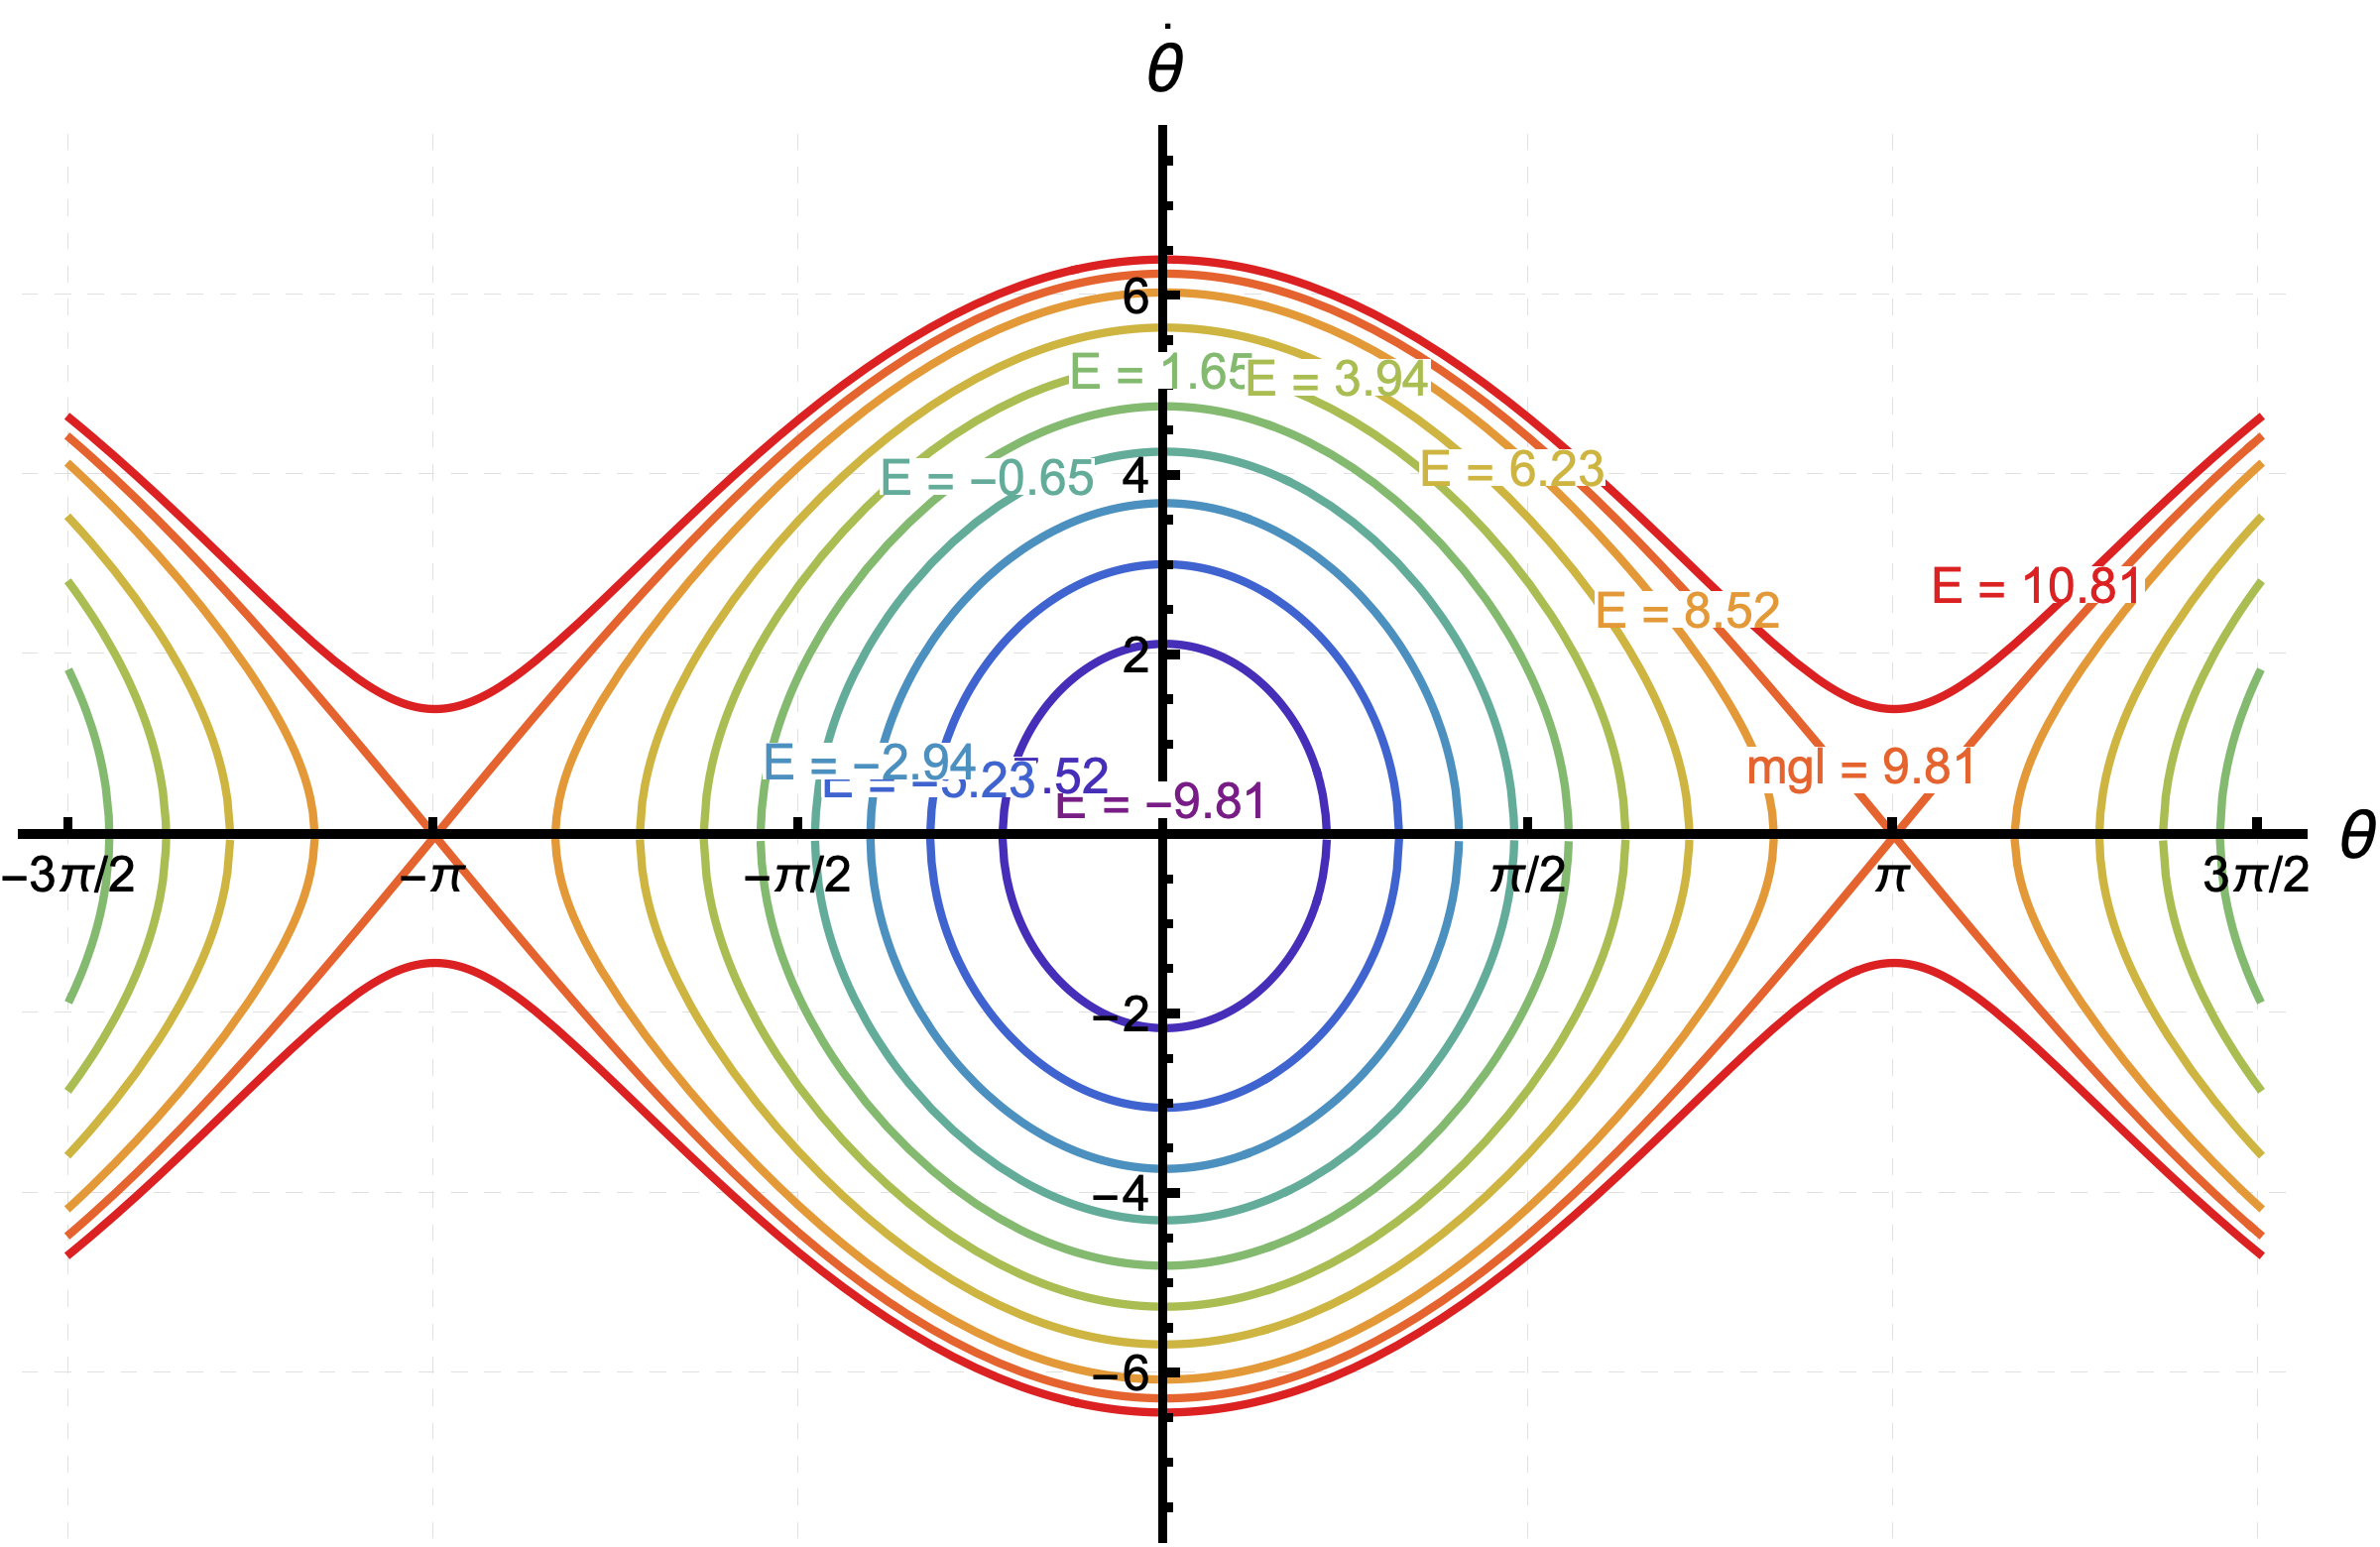
\includegraphics[width=0.62\linewidth]{immagini/grafico_pendolo}
\end{center}

La curva ad energia \(E=mg\ell\) si chiama curva separatrice

\[
E<E_0=mg\ell
\qquad
\text{orbite chiuse}
\]

\[
E>E_0=mg\ell
\qquad
\text{orbite aperte}
\]

Notiamo che il verso di percorrenza di queste curve dipende dalle condizioni iniziali. Nel piano delle fasi

\[
\begin{cases}
x=\theta\\
y=\dot{\theta}
\end{cases}
\Rightarrow
\begin{cases}
\dot{x}=\dot{\theta}\\
\dot{y}=\ddot{\theta}=-\omega^2\sin\theta
\end{cases}
\]

Allora
\[
\vec{v}=(\dot{\theta},-\omega^2\sin\theta)
\]
ovvero il segno di \(\dot{\theta}\) mi dice se mi muovo a destra o a sinistra e il segno di \(-\omega^2\sin\theta\) mi dice se mi muovo in alto o in basso.\\
Se $\dot \theta > 0 $ le curve vengono percorse verso destra mentre se $\dot \theta < 0$ vengono percorse verso sinistra. Inoltre se
\[
\sin \theta < 0 \quad \Leftrightarrow - \pi + 2k \pi < \theta < 2 k \pi
\]
le curve vengono percorse verso l'alto mentre se
\[
\sin \theta > 0 2k \pi < \theta < \pi + 2k \pi
\]
le curve vengono percorse verso il basso.\\
In conclusione se $E < mgl$ le curve chiuse vengono percorse in senso orario mentre se $E > mgl$ le curve aperte vengono percorse verso destra se $\dot \theta> 0$ e verso sinistra se $\dot \theta < 0$.\\
Analizziamo ora il periodo del pendolo. Nel caso lineare

\[
\theta\ll 1
\qquad
\sin\theta\sim\theta
\qquad
\theta(t)=A\cos(\omega t+\varphi)
\qquad
\omega^2=\frac{g}{\ell}
\Rightarrow
T=\frac{2\pi}{\omega}=2\pi\sqrt{\frac{\ell}{g}}
\]

Questa è detta isocronia delle piccole oscillazioni ed è attribuita a Galileo.

Nel caso non lineare

\[
\ddot{\theta}=-\omega^2\sin\theta
\Rightarrow
\dot{\theta}\ddot{\theta}=-\omega^2\sin\theta\dot{\theta}
\Rightarrow
\frac{d}{dt}\left(\frac{\dot{\theta}^2}{2}\right)
=
-\omega^2\frac{d}{dt}(-\cos\theta)
\]

\[
\Rightarrow
\frac{E}{m\ell^2}
=
\frac{\dot{\theta}^2}{2}-\omega^2\cos\theta
=
\left.\frac{\dot{\theta}^2}{2}\right|_{t=0}
-
\left.\omega^2\cos\theta\right|_{t=0}
\]

Chiamo
\[
\mathcal{E}=\frac{E}{m\ell^2}
\]

\[
\Rightarrow
\frac{\dot{\theta}^2}{2}=\mathcal{E}+\omega^2\cos\theta
\Rightarrow
\dot{\theta}^2=2(\mathcal{E}+\omega^2\cos\theta)
\Rightarrow
\dot{\theta}=\pm\sqrt{2}\cdot\sqrt{\mathcal{E}+\omega^2\cos\theta}
\]

Scelgo una traiettoria da \(-\theta_0\) a \(\theta_0\) e quindi \(\dot{\theta}>0\) ovvero

\[
\dot{\theta}
=
\sqrt{2}\cdot\sqrt{\mathcal{E}+\omega^2\cos\theta}
=
\frac{d\theta}{dt}
\]

Abbiamo trovato una EDO a variabili separabili. La integro tra \(0\) e \(T/2\) perché integrare da \(0\) a \(T\) implicherebbe integrare tra \(-\theta_0\) e \(-\theta_0\).

\[
\frac{d\theta}{\sqrt{2}\sqrt{\mathcal{E}+\omega^2\cos\theta}}=dt
\Rightarrow
\int_{0}^{T/2}dt=\frac{T}{2}
=
\int_{-\theta_0}^{\theta_0}
\frac{d\theta}{\sqrt{2}\sqrt{\mathcal{E}+\omega^2\cos\theta}}
\]

\[
\Rightarrow
T
=
\sqrt{2}
\int_{-\theta_0}^{\theta_0}
\frac{d\theta}{\sqrt{\mathcal{E}+\omega^2\cos\theta}}
\]

Per oscillazioni chiuse si ha che per \(\theta=\theta_0\), \(\dot{\theta}=0\) ovvero

\[
\mathcal{E}=-\omega^2\cos\theta_0.
\]

Sostituendo in \(T\) si ottiene

\[
T
=
\sqrt{2}
\int_{-\theta_0}^{\theta_0}
\frac{d\theta}{\sqrt{\omega^2(\cos\theta-\cos\theta_0)}}
=
\frac{\sqrt{2}}{\omega}
\int_{-\theta_0}^{\theta_0}
\frac{d\theta}{\sqrt{\cos\theta-\cos\theta_0}}
=
\sqrt{2}\sqrt{\frac{\ell}{g}}
\int_{-\theta_0}^{\theta_0}
\frac{d\theta}{\sqrt{\cos\theta-\cos\theta_0}}
\]

Nel caso lineare
\[
\cos\theta\sim 1-\frac{\theta^2}{2}
\qquad
\cos\theta_0\sim 1-\frac{\theta_0^2}{2}
\Rightarrow
\cos\theta-\cos\theta_0=\frac{\theta_0^2-\theta^2}{2}
\]

Allora

\[
T
\sim
2\sqrt{\frac{\ell}{g}}
\int_{-\theta_0}^{\theta_0}
\frac{d\theta}{\sqrt{\theta_0^2-\theta^2}}
=
2\sqrt{\frac{\ell}{g}}
\arcsin\left(\frac{\theta}{\theta_0}\right)\Big|_{-\theta_0}^{\theta_0}
\]

\[
=
2\sqrt{\frac{\ell}{g}}
\left(\arcsin(1)-\arcsin(-1)\right)
=
2\sqrt{\frac{\ell}{g}}
\left(\frac{\pi}{2}-\left(-\frac{\pi}{2}\right)\right)
,
\,
2\pi\sqrt{\frac{\ell}{g}}
\]

Ovvero abbiamo ritrovato il periodo del pendolo linearizzato.
\end{example}
Consideriamo un sistema conservativo ad \(1\) grado di libertà. Posso scrivere
\[
T=\frac{1}{2}a(q)\dot q^2
\qquad
V=V(q)
\]

Sia \((q,\dot q)=(q_0,0)\) una configurazione di equilibrio, ovvero un minimo di \(V(q)\).

Vogliamo linearizzare le equazioni del moto attorno alla configurazione di equilibrio.

Sviluppo \(V(q)\)
\[
V(q)
=
V(q_0)+V'(q_0)(q-q_0)+\frac{V''}{2}(q_0)(q-q_0)^2+o(q-q_0)^2
\]

Visto che le costanti sono arbitrarie per un potenziale pongo \(V(q_0)=0\) ed inoltre \(V'(q_0)(q-q_0)=0\) perché \(q_0\) è un punto di minimo (Fermat). Per lo stesso motivo \(V''(q_0)>0\). Allora
\[
V(q)=\frac{V''}{2}(q_0)(q-q_0)^2+o(q-q_0)^2
\]

Allo stesso modo l'energia cinetica
\[
2T=a(q)\dot q^2
=
a(q_0)\dot q^2
+
\left.
\begin{pmatrix}
a'(q)\dot q^2\\
a(q)\cdot 2\dot q
\end{pmatrix}
\right|_{(q,\dot q)=(q_0,0)}
\cdot
\binom{q-q_0}{\dot q}
\]
\[
+
\frac{1}{2}
\begin{pmatrix}
q-q_0\\
\dot q
\end{pmatrix}^{T}
\cdot
\left.
\begin{pmatrix}
a''(q)\dot q^2 & 2a'(q)\dot q\\
a'(q)\cdot 2\dot q & 2a(q)
\end{pmatrix}
\right|_{(q,\dot q)=(q_0,0)}
\cdot
\binom{q-q_0}{\dot q}
+
o\left(
\left\|
\binom{q-q_0}{\dot q}
\right\|^2
\right)
=
\]
\[
=
\frac{1}{2}
\begin{pmatrix}
q-q_0\\
\dot q
\end{pmatrix}^{T}
\cdot
\begin{pmatrix}
0 & 0\\
0 & 2a(q_0)
\end{pmatrix}
\cdot
\binom{q-q_0}{\dot q}
+
o\left(
\left\|
\binom{q-q_0}{\dot q}
\right\|^2
\right)
=
\]
\[
=
\frac{1}{2}
\begin{pmatrix}
q-q_0\\
\dot q
\end{pmatrix}^{T}
\cdot
\binom{0}{2a(q_0)\dot q}
+
o\left(
\left\|
\binom{q-q_0}{\dot q}
\right\|^2
\right)
=
\]
\[
=
a(q_0)\dot q^2
+
o\left(
\left\|
\binom{q-q_0}{\dot q}
\right\|^2
\right)
\Rightarrow
T\simeq \frac{1}{2}a(q_0)\dot q^2
\]

La lagrangiana linearizzata è quindi
\[
\tilde{\mathcal{L}}
=
\frac{1}{2}a(q_0)\dot q^2
-
\frac{V''}{2}(q_0)(q-q_0)^2
\]

Scriviamo le equazioni di Lagrange del problema linearizzato
\[
\frac{\partial \tilde{\mathcal{L}}}{\partial \dot q}
=
a(q_0)\dot q
\Rightarrow
\frac{d}{dt}\frac{\partial \tilde{\mathcal{L}}}{\partial \dot q}
=
a(q_0)\ddot q,
\qquad
\frac{\partial \tilde{\mathcal{L}}}{\partial q}
=
-
V''(q_0)(q-q_0)
\]
\[
\Rightarrow
a(q_0)\ddot q=-V''(q_0)(q-q_0)
\]

Ponendo \(t=q-q_0\Rightarrow \ddot t=\ddot q\) otteniamo
\[
\ddot t=-\omega^2t,
\qquad
\omega^2=\frac{V''(q_0)}{a(q_0)}
\qquad
a(q_0)>0 \text{ perché } T>0
\]

Ogni sistema ad \(1\) G.D.L. vicino ad una configurazione di equilibrio stabile si comporta come un oscillatore armonico.
Linearizziamo ora le equazioni del moto per un sistema conservativo con \(m\) gradi di libertà.
Siano \(\{q_1,\ldots,q_m\}\) le coordinate libere.

Per il sistema possiamo scrivere
\[
V(\underline q),
\qquad
T(\underline q,\dot{\underline q})
=
\frac{1}{2}\dot{\underline q}^{T}A(\underline q)\dot{\underline q}
\qquad
\text{con } A(\underline q) \text{ definita positiva}
\]
sia
\[
(\underline q,\dot{\underline q})=(\underline q_0,\underline 0)
\]
configurazione di equilibrio stabile.

Scriviamo lo sviluppo di Taylor per \(V(\underline q)\)
\[
V(\underline q)
=
V(\underline q_0)
+
\nabla V\big|_{\underline q_0}\cdot(\underline q-\underline q_0)
+
\frac{1}{2}(\underline q-\underline q_0)^{T}
H(V)\big|_{\underline q_0}\cdot(\underline q-\underline q_0)
+
o\left(\|\underline q-\underline q_0\|^2\right)
\]

Per gli stessi motivi del caso \(m=1\) possiamo porre \(V(\underline q_0)=0\) e
\[
\nabla V(\underline q_0)=\underline 0.
\]
Inoltre \(H_V(\underline q_0)\) è definita positiva.

Con ragionamenti analoghi al caso \(m=1\) otteniamo
\[
T\sim \frac{1}{2}\dot{\underline q}^{T}A(\underline q_0)\dot{\underline q}
\]
con \(A(\underline q_0)\) definita positiva.

Poniamo $\underline{t} = \underline{q} - \underline{q_0}$. La lagrangiana per il sistema è
\[
\tilde{\mathcal{L}}
=
\frac{1}{2}\dot{\underline t}^{T}A\dot{\underline t}
-
\frac{1}{2}\underline t^{T}H_V\underline t
=
\sum_{i=1}^{m}\sum_{j=1}^{m}
a_{ij}(\underline t_0)\frac{\dot t_i\dot t_j}{2}
-
\sum_{i=1}^{m}\sum_{j=1}^{m}
\frac{H_{ij}}{2}t_it_j
\]

Allora
\[
\frac{\partial\tilde{\mathcal{L}}}{\partial\dot t_j}
=
\sum_{i=1}^{m}a_{ij}\big|_{\underline t_0}\cdot\dot t_i
\qquad
\frac{d}{dt}\frac{\partial\tilde{\mathcal{L}}}{\partial\dot t_j}
=
\sum_{i=1}^{m}a_{ij}(\underline t_0)\ddot t_i
\]
\[
\frac{\partial\tilde{\mathcal{L}}}{\partial t_j}
=
-\sum_{i=1}^{m}H_{ij}t_i
\]

\[
\Rightarrow
\sum_{i=1}^{m}a_{ij}\ddot t_i
=
-\sum_{i=1}^{m}H_{ij}t_i
\qquad
\forall j=1,\ldots,m
\]

o in forma compatta
\[
A\ddot{\underline t}=-H\underline t
\]

\[
A=\{a_{ij}\},
\qquad
H=
\left\{
\left.
\frac{\partial^2 V}{\partial t_i\partial t_j}
\right|_{\underline t_0}
\right\}
\]
sono simmetriche definite positive \(\Rightarrow\) hanno autovalori reali positivi \(\Rightarrow\) sono invertibili. Allora
\[
\ddot{\underline t}=-A^{-1}H\underline t
\]

\begin{oss}{}
Il prodotto di \(2\) matrici simmetriche non è simmetrico
\[
(AB)^{T}=B^{T}A^{T}=BA\neq AB
\]

ma vale la seguente.
\end{oss}
\begin{lemma}{}
Siano \(A, B\) simmetriche e definite positive. Allora \(AB\) è diagonalizzabile e ha autovalori reali positivi.
\end{lemma}
\begin{proof}
Consideriamo
\[
A^{-1/2}ABA^{1/2}=A^{1/2}BA^{1/2}.
\]
Si osserva che
\[
\text{(i) è simmetrica:}\quad
\left(A^{-1/2}ABA^{1/2}\right)^T
=
\left(A^{1/2}\right)^T \cdot \left(A^{-1/2}AB\right)^T
=
A^{1/2}(AB)^T\left(A^{-1/2}\right)^T
=
A^{1/2}B^TA^TA^{-1/2}
=
\]
\[
=
A^{1/2}BAA^{-1/2}
=
A^{1/2}BA^{1/2}.
\]
\[
\text{(ii) è definita positiva:}\quad
\underline{x}^T A^{-1/2}ABA^{1/2}\underline{x}
=
\underline{x}^T A^{1/2}BA^{1/2}\underline{x}
=
\underline{x}^T\left(A^{1/2}\right)^TBA^{1/2}\underline{x}
=
\]
\[
=
\left(A^{1/2}\underline{x}\right)^TBA^{1/2}\underline{x}
=
\underline{y}^TB\underline{y}\ge 0
\quad \forall \underline{y}\in \mathbb{R}^n
\]
con
\[
\underline{y}=A^{1/2}\underline{x}.
\]
Ci ricordiamo che 2 matrici simili hanno gli stessi autovalori e notiamo che
\[
\left(A^{1/2}\right)^{-1}ABA^{1/2}\sim AB.
\]
Concludiamo che \(AB\) è diagonalizzabile e ha 2 autovalori positivi.
\end{proof}

Voglio diagonalizzare
\[
A^{-1}H=B.
\]
Considero \(P\) la matrice che ha come colonne gli autovettori di \(B\), \(D\) diagonale con autovalori sulla diagonale. Vale
\[
BP=PD
\Rightarrow
P^{-1}\ddot{\underline t}=-P^{-1}B\underline t
\]

Chiamo
\[
P\underline v=\underline t
\]

\[
\Rightarrow
P^{-1}(P\ddot{\underline v})
=
-P^{-1}BP\underline v
\Rightarrow
\ddot{\underline v}
=
-D\underline v
\Longleftrightarrow
\ddot v_i=-\lambda_i v_i
\qquad
\forall i=1,\ldots,m
\]

Le \(t_i\) sono una combinazione lineare delle \(v_i\) tramite \(P\).
Sono riuscito a scrivere il moto come una combinazione di oscillatori armonici.
\begin{example}{}
Studiamo il seguente sistema per piccole oscillazioni

\[
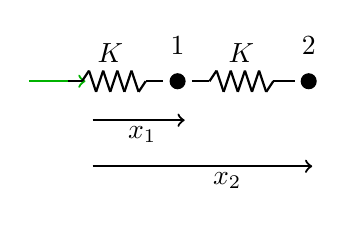
\begin{tikzpicture}[scale=0.9]
  \draw[green!70!black, thick, ->] (-0.2,0.4) -- (0.6,0.4);

  \draw[thick] (0.35,0.4) -- (0.55,0.4);
  \draw[thick] (0.55,0.4) -- (0.65,0.55);
  \draw[thick] (0.65,0.55) -- (0.75,0.25);
  \draw[thick] (0.75,0.25) -- (0.85,0.55);
  \draw[thick] (0.85,0.55) -- (0.95,0.25);
  \draw[thick] (0.95,0.25) -- (1.05,0.55);
  \draw[thick] (1.05,0.55) -- (1.15,0.25);
  \draw[thick] (1.15,0.25) -- (1.25,0.55);
  \draw[thick] (1.25,0.55) -- (1.35,0.25);
  \draw[thick] (1.35,0.25) -- (1.45,0.4);
  \draw[thick] (1.45,0.4) -- (1.7,0.4);

  \filldraw[black] (1.9,0.4) circle (3pt);
  \node at (1.9,0.9) {$1$};
  \node at (0.95,0.8) {$K$};

  \draw[thick] (2.1,0.4) -- (2.35,0.4);
  \draw[thick] (2.35,0.4) -- (2.45,0.55);
  \draw[thick] (2.45,0.55) -- (2.55,0.25);
  \draw[thick] (2.55,0.25) -- (2.65,0.55);
  \draw[thick] (2.65,0.55) -- (2.75,0.25);
  \draw[thick] (2.75,0.25) -- (2.85,0.55);
  \draw[thick] (2.85,0.55) -- (2.95,0.25);
  \draw[thick] (2.95,0.25) -- (3.05,0.55);
  \draw[thick] (3.05,0.55) -- (3.15,0.25);
  \draw[thick] (3.15,0.25) -- (3.25,0.4);
  \draw[thick] (3.25,0.4) -- (3.55,0.4);

  \filldraw[black] (3.75,0.4) circle (3pt);
  \node at (3.75,0.9) {$2$};
  \node at (2.8,0.8) {$K$};

  \draw[->, thick] (0.7,-0.15) -- (2.0,-0.15);
  \node at (1.4,-0.35) {$x_1$};

  \draw[->, thick] (0.7,-0.8) -- (3.8,-0.8);
  \node at (2.6,-1) {$x_2$};
\end{tikzpicture}
\]

Il sistema ha 2 gradi di libertà. Scegliamo come coordinate libere \(x_1,x_2\). Scriviamo l'energia cinetica del sistema.
\[
T = m\frac{\dot{x}_1^2}{2} + m\frac{\dot{x}_2^2}{2}
=
\frac{1}{2}
(\dot{x}_1,\dot{x}_2)
\begin{pmatrix}
m & 0\\
0 & m
\end{pmatrix}
\begin{pmatrix}
\dot{x}_1\\
\dot{x}_2
\end{pmatrix}
\]
È una forma quadratica definita positiva e quindi
\[
H_T=
\begin{pmatrix}
m & 0\\
0 & m
\end{pmatrix}.
\]
Studiamo l'energia potenziale del sistema.
\[
V(x_1,x_2)=\frac{K}{2}x_1^2+\frac{K}{2}(x_2-x_1)^2
\Rightarrow
\nabla V(x_1,x_2)=
\left(
\frac{\partial V}{\partial x_1}(x_1,x_2),
\frac{\partial V}{\partial x_2}(x_1,x_2)
\right)
=
\]
\[
=
\left(
Kx_1-K(x_2-x_1),K(x_2-x_1)
\right)
\]
I punti di equilibrio stabile sono i minimi di \(V\). Annulliamo \(\nabla V(x_1,x_2)\)
\[
\begin{cases}
K(x_2-x_1)=0 \Rightarrow x_1=x_2\\
K(2x_1-x_2)=0 \Rightarrow Kx_1=0 \Rightarrow x_1=x_2=0
\end{cases}
\]
Allora \((0,0)\) è l'unico candidato di configurazione di equilibrio statico. Studiamo l'Hessiana.
\[
\frac{\partial^2 V}{\partial x_1^2}=2K
\qquad
\frac{\partial^2 V}{\partial x_2^2}=K
\qquad
\frac{\partial^2 V}{\partial x_1\partial x_2}=-K
\Rightarrow
H_V=
\begin{pmatrix}
2K & -K\\
-K & K
\end{pmatrix}
=
K
\begin{pmatrix}
2 & -1\\
-1 & 1
\end{pmatrix}
\]
Ricordiamo che se \(f\) è un'applicazione lineare e \(f(v)=\lambda v\) allora
\[
\alpha f(v)=\alpha \lambda v
\]
ovvero gli autovalori di \(\alpha f\) sono i \(\alpha \lambda_i\) con \(\lambda_i\) autovalori di \(f\). Calcoliamo gli autovalori di
\[
\begin{pmatrix}
2 & -1\\
-1 & 1
\end{pmatrix}
\]
\[
\det
\begin{pmatrix}
2-\lambda & -1\\
-1 & 1-\lambda
\end{pmatrix}
=
(2-\lambda)(1-\lambda)-1
=
2-2\lambda-\lambda+\lambda^2-1
=
\lambda^2-3\lambda+1
\]
\[
\lambda^2-3\lambda+1=0
\Leftrightarrow
\lambda=
\frac{3\pm\sqrt{9-4}}{2}
=
\frac{3\pm\sqrt{5}}{2}
\]
Gli autovalori di \(H_V\) sono quindi
\[
\lambda_1=\frac{3-\sqrt{5}}{2}K,
\qquad
\lambda_2=\frac{3+\sqrt{5}}{2}K.
\]
In particolare \(H_V\) è definita positiva in \((0,0)\) che è quindi un punto di minimo di \(V\).

Linearizziamo il problema attorno a \((0,0)\)
\[
\mathcal{L}(\underline{x},\dot{\underline{x}})
\sim
\frac{1}{2}
(\dot{x}_1,\dot{x}_2)^T
\begin{pmatrix}
m & 0\\
0 & m
\end{pmatrix}
\begin{pmatrix}
\dot{x}_1\\
\dot{x}_2
\end{pmatrix}
-
\frac{1}{2}
(x_1,x_2)
\begin{pmatrix}
2K & -K\\
-K & K
\end{pmatrix}
\begin{pmatrix}
x_1\\
x_2
\end{pmatrix}
\]
Nelle notazioni precedenti
\[
A=
\begin{pmatrix}
m & 0\\
0 & m
\end{pmatrix}
\qquad
H=
\begin{pmatrix}
2K & -K\\
-K & K
\end{pmatrix}
\]
\[
B=A^{-1}H
=
\begin{pmatrix}
\frac{1}{m} & 0\\
0 & \frac{1}{m}
\end{pmatrix}
\cdot
\begin{pmatrix}
2K & -K\\
-K & K
\end{pmatrix}
=
\begin{pmatrix}
\frac{2K}{m} & -\frac{K}{m}\\
-\frac{K}{m} & \frac{K}{m}
\end{pmatrix}
=
\frac{K}{m}
\begin{pmatrix}
2 & -1\\
-1 & 1
\end{pmatrix}
\]
Gli autovalori di \(B\) sono
\[
\lambda_1=\frac{3-\sqrt{5}}{2}\frac{K}{m},
\qquad
\lambda_2=\frac{3+\sqrt{5}}{2}\frac{K}{m}
\]
\(\lambda_{1,2}\) sono entrambe positive e sono le frequenze proprie di oscillazione attorno all'equilibrio.
\end{example}

\begin{example}{}
Tutti i vincoli sono di puro scivolamento. Trovare il valore minimo di \(K\) perché il sistema resti in equilibrio.

\[
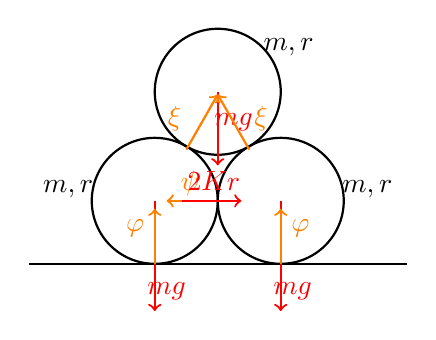
\begin{tikzpicture}[scale=1]
  \draw[thick] (-2.4,0) -- (2.4,0);

  \draw[thick] (-0.8,0.8) circle (0.8);
  \draw[thick] (0.8,0.8) circle (0.8);
  \draw[thick] (0,2.185) circle (0.8);


  \node at (-1.9,0.95) {\(m,r\)};
  \node at (1.9,0.95) {\(m,r\)};
  \node at (0.9,2.75) {\(m,r\)};

  \draw[red, thick, ->] (-0.8,0.8) -- (-0.8,-0.6);
  \node[red] at (-0.65,-0.35) {\(mg\)};

  \draw[red, thick, ->] (0.8,0.8) -- (0.8,-0.6);
  \node[red] at (0.95,-0.35) {\(mg\)};

  \draw[red, thick, ->] (0,2.185) -- (0,1.25);
  \node[red] at (0.2,1.8) {\(mg\)};

  \draw[orange, thick, ->] (-0.8,0) -- (-0.8,0.7);
  \node[orange] at (-1.05,0.45) {\(\varphi\)};

  \draw[orange, thick, ->] (0.8,0) -- (0.8,0.7);
  \node[orange] at (1.05,0.45) {\(\varphi\)};

  \draw[orange, thick, ->] (-0.4,1.45) -- (0,2.15);
  \node[orange] at (-0.55,1.85) {\(\xi\)};

  \draw[orange, thick, ->] (0.4,1.45) -- (0,2.15);
  \node[orange] at (0.55,1.85) {\(\xi\)};

  \draw[orange, thick, ->] (0,0.8) -- (-0.65,0.8);
  \node[orange] at (-0.35,1.02) {\(\psi\)};

  \draw[red, thick, ->] (-0.45,0.8) -- (0.3,0.8) ;
  \node[red] at (-0.05,1.05) {\(2Kr\)};


\end{tikzpicture}
\]

\begin{itemize}
  \item Bilancio delle forze su tutto il sistema
  \[
  2\varphi - 3mg = 0 \Rightarrow \varphi = \frac{3}{2}mg
  \]

  \item Bilancio delle forze disco 1 direzione orizzontale
  \[
  2Kr + \psi + \xi \cos \frac{\pi}{3} = 0
  \]

  \item Bilancio delle forze disco 1 direzione verticale
  \[
  \xi \sin \frac{\pi}{3} + \varphi - mg = 0
  \Rightarrow
  -mg + \frac{3}{2}mg = -\xi \sin \frac{\pi}{3}
  \Rightarrow
  \xi =
  \frac{-mg}{2\sin \frac{\pi}{3}}
  =
  -\frac{mg}{\sqrt{3}}
  \]
\end{itemize}

\[
\Rightarrow
\psi =
-2Kr - \xi \cos \frac{\pi}{3}
=
-2Kr + \frac{mg}{\sqrt{3}}\cdot \frac{1}{2}
=
-2Kr + \frac{mg}{2\sqrt{3}}
\]

\[
\text{Se } \psi = 0
\Rightarrow
2K_{\min}r = \frac{mg}{2\sqrt{3}}
\Rightarrow
K_{\min} = \frac{mg}{4\sqrt{3}r}
\]
\end{example}
